% Document settings
\documentclass[a4paper,11pt]{article}

% Packages
  % math formulas
\usepackage{amsmath,amsthm,amssymb}
  % graphics
\usepackage{graphicx}
\usepackage{wrapfig}
  % plots
\usepackage{pgfplots}
  % other
\usepackage[warn]{mathtext}
\usepackage{cmap}
\usepackage[T1,T2A]{fontenc}
\usepackage[utf8]{inputenc}
\usepackage[english,russian]{babel}

% Package settings
%% graphicx
\graphicspath{{Pictures/}}
\DeclareGraphicsExtensions{.pdf,.png,.jpg}
%% pgfplots
\pgfplotsset{width=10cm,compat=1.9}

% Title
\title{Отчет о выполнении работы №1.3.3\\Измерение вязкости воздуха при течении в тонких трубках}
\author{Воейко Андрей Александрович, Б01-109}
\date{Долгопрудный, 2022}

% Document
\begin{document}
\maketitle
\newpage
\section{Аннотация.}
В работе экспериментально исследуется свойства течения газов по тонким трубкам, а также выявляется область применимости закона Пуассона и с его помощью определяется коэффицент вязкости воздуха.
\section{Теоретические сведения.}
Движение жидкости или газа в трубке вызвается перепадом внешнего давления $\Delta P$ на концах. Препятствуют движению силы вязкого трения, действующие между соседними слоями жидкости, а также со стороны стенок трубы. Сила вязкого трения в жидкостях и газах описывается законом Ньютона. В частности, если жидкость течет вдоль оси x, а скорость течения $v_{x}(y)$ зависит от координты и $y$, в каждом слое возникает направленное по $x$ касательное напряжение:
\begin{equation}    \label{eq1}
  \tau_{xy} = -\eta \frac{\delta v_{x}}{\delta y},
\end{equation}
Где $\tau_{xy}$ -- касательное напряжение, $\eta$ -- коэффицент динамической вязкости среды.
Характер течения в трубе может быть ламинарным -- когда слои жидкости или газа не перемешиваются между собой, и турбулентным -- когда они перемешиваются. Определяется числом Рейнольдса:
\begin{equation}    \label{eq2}
  Re = \frac{\rho u R}{\eta},
\end{equation}
где $\rho$ -- плотность среды, $u$ -- характерная скорость потока, $a$ -- характерный размер системы (размер, на котором существенно меняется скорость течения). Из опыта известно, что переход к турбулентному течению для трубок круглого сечения наблюдается при $Re_{кр} \approx 10^{3}$.\\
В целях упрощения теоретической модели газа в услоаиях экспериента можно считать несжимаемым, то есть принять плотность среды постоянной: $\rho = const$. Для газов такое приближение допустимо, если относительный перепад давления в трубе мал: $\Delta P \ll P$.
Расход воздуха найдем по формуле Пуазейля:
\begin{equation}    \label{eq3}
  Q = \frac{\pi R^{4} \Delta P}{8 \eta l},
\end{equation}
где $R$ -- радиус трубки, $l$ -- длина отрезка трубки. При этом, чтобы движение стало Пуазейлевским, необходимо, чтобы оно установилось. Длина установления вычисляется по формуле:
\begin{equation}    \label{eq4}
  l_{уст} \approx 0,2 R \cdot Re.
\end{equation}
При турбулентном течении расход будет определяться по такой формуле:
\begin{equation}    \label{eq5}
  Q = \pi R^{2} \overline {u} \sim R^{\frac{5}{2}} \sqrt {\frac{\Delta P}{\rho l}\ }.
\end{equation}
\section{Оборудование.}
\subsection{Импользуемое оборудование.}
В работе используются:
\begin{itemize}
  \item компрессор и проводящие трубки для подвода воздуха
  \item газовый счетчик. Диапазон измерений -- $5\ л$. Цена деления -- $0,02\ л$
  \item спиртовой манометр с регулируемым наклоном. Угол наклона использовался такой, что его $\sin$ равен $0,2$
  \item трубка диаметра примерно $\ мм$
\end{itemize}
\subsection{Описание экспериментальная установка.}
Экспериментальная установка изображена на рисунке~\ref{fig:img1}.
\begin{wrapfigure}{r}{0.7\textwidth}
  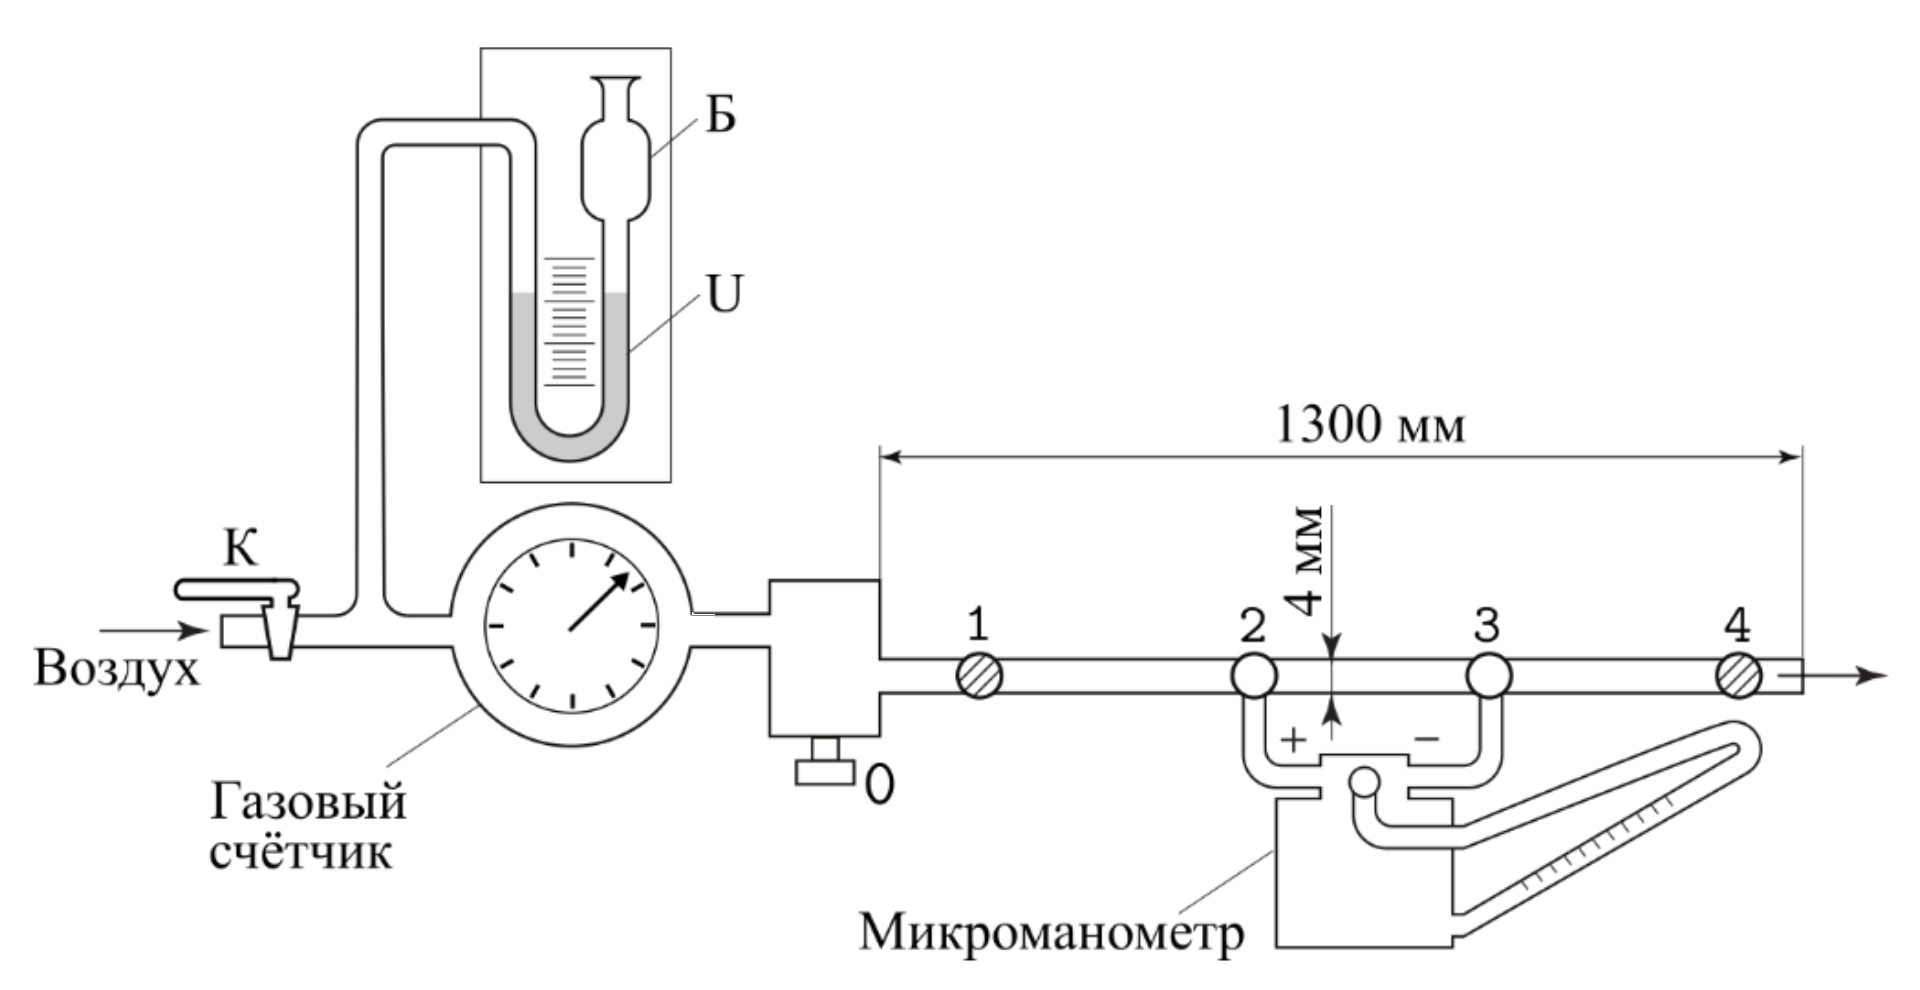
\includegraphics[scale = 0.224]{scheme1.png}
  \caption{Схема экспериментальной установки.}
  \label{fig:img1}
\end{wrapfigure}
Трубка имеет несколько отверстий, которые либо закрываются заглушками, либо подключаются к микроманометру. Один конец открыт, другой поключен к системе подачи воздуха. Сама подача воздуха регулируется краном К. К ней же подключен маслянный U-образный манометр с бачком Б, который издает заметный звук при превышении определенного значения. Расход воздуха измеряется газовым счетчиком.
\section{Результаты измерений и и обработка данных.}
\subsection{Предварительные вычисления.}
Вычислим такой расход воздуха, при котором число Рейнольдса $Re$ будет примерно равна $10^{3}$:
$$ Re = \frac{\rho \overline{u} R}{\eta} \Rightarrow \overline{u} = \frac{Re \cdot \eta}{\rho R}.$$
$$ \overline{u} = \frac{Q_{кр}}{\pi R^{2}} = \frac{Re \cdot \eta}{\rho R} \Rightarrow Q_{кр} = \pi R \cdot \frac{Re \cdot \eta}{\rho}.$$
$$Q_{кр} = 0,106\ \frac{л}{с} = 2,96\ \frac{л}{мин}.$$
Теперь найдем критическое $\Delta P$, при котором ламинарное течение переходит в турбулентное:
$$\Delta P = 177\ Па.$$
Далее найдем $l_{уст}$:
$$l_{уст} = 0,395\ м.$$
\subsection{Результаты измерений.} %%%%% Результаты измерений %%%%%
\subsubsection{Измерение зависимости перепада давления $\Delta P$ от расхода газа $Q$.}
Проведем измерения $\Delta P$ от $Q$ на длине $131,2\ мм$. Результаты занесем в таблицу. Результаты измерений представлены в таблице~\ref{table:tab1}.
% Начало таблицы 1 {{{
\begin{table}[h!]
\centering
\begin{tabular}{ ||c|c|c|c|c|c|| }
  \hline
  № & Объем, $л$ & Время, $с$ & $Q$, $\cdot 10^{-3}\ \frac{л}{с}$ & $\Delta P$, $дел$ & $\Delta P$, $Па$ \\
  \hline
  \multicolumn{6}{||c||}{Ламинарный поток} \\
  \hline
  1 & $2 \pm 0,02$ & $49,8 \pm 0,6$ & $40,2 \pm 0,9$ & $30 \pm 1$ & $58,9 \pm 1,96$ \\
  2 & $3 \pm 0,02$ & $58,5 \pm 0,6$ & $51,3 \pm 0,9$ & $40 \pm 1$ & $78,5 \pm 1,96$ \\
  3 & $4 \pm 0,02$ & $61,2 \pm 0,6$ & $65,4 \pm 1,0$ & $51 \pm 1$ & $100,1 \pm 1,96$ \\
  4 & $4 \pm 0,02$ & $54,3 \pm 0,6$ & $73,7 \pm 1,2$ & $56 \pm 1$ & $109,9 \pm 1,96$ \\
  5 & $5 \pm 0,02$ & $64,9 \pm 0,6$ & $77,0 \pm 1,0$ & $60 \pm 1$ & $117,7 \pm 1,96$ \\
  6 & $6 \pm 0,02$ & $67,3 \pm 0,6$ & $89,2 \pm 1,1$ & $69 \pm 1$ & $135,4 \pm 1,96$ \\
  \hline
  \multicolumn{6}{||c||}{Турбулентный поток} \\
  \hline
  7 &  $6 \pm 0,02$  & $58,4 \pm 0,6$ & $102,7 \pm 0,9$ & $95 \pm 1$  & $186,4 \pm 1,96$ \\
  8 & $6,5 \pm 0,02$ & $63,0 \pm 0,6$ & $103,2 \pm 0,9$ & $99 \pm 1$  & $194,3 \pm 1,96$ \\
  9 &  $7 \pm 0,02$  & $64,7 \pm 0,6$ & $108,2 \pm 0,9$ & $122 \pm 1$ & $239,4 \pm 1,96$ \\
  10 & $7 \pm 0,02$  & $62,5 \pm 0,6$ & $112,0 \pm 0,9$ & $130 \pm 1$ & $255,2 \pm 1,96$ \\
  11 & $7 \pm 0,02$  & $61,9 \pm 0,6$ & $113,1 \pm 0,9$ & $143 \pm 1$ & $280,6 \pm 1,96$ \\
  12 & $8 \pm 0,02$  & $68,7 \pm 0,6$ & $116,4 \pm 0,9$ & $150 \pm 1$ & $294,3 \pm 1,96$ \\
  13 & $8 \pm 0,02$  & $65,7 \pm 0,6$ & $121,8 \pm 0,9$ & $165 \pm 1$ & $323,7 \pm 1,96$ \\
  \hline
\end{tabular}
\caption{Результаты измерения зависимости $\Delta P$ от $Q$.}
\label{table:tab1}
\end{table}
% }}} Конец таблицы 1
\subsubsection{Измерение зависимости перепада давления $\Delta P$ от длины отрезка трубки.}
Проведем измерения $\Delta P$ от $Q$ на длине $131,2\ мм$. Результаты измерений представлены в таблице~\ref{table:tab1}. В ней в шапке и первом столбце обозначено расстояние от начала трубки до отверстия, а в теле таблицы в первой части -- разница давлений в делениях, а во второй -- в паскалях.
% Начало таблицы 2 {{{
\begin{table}[h!]
\centering
\begin{tabular}{ ||c|c|c|c|c|c|| }
  \hline
  \multicolumn{6}{||c||}{Разница давлений в делениях} \\
  \hline
   & $0$ & $11,2$ & $41,2$ & $81,2$ & $131,2$ \\
  \hline
   $0$   & -- & $59$ & $110$ & $177$ & $246$ \\
  $11,2$ & -- &  --  & $51$  & $119$ & $187$ \\
  $41,2$ & -- &  --  &  --   & $66$  & $135$ \\
  $81,2$ & -- &  --  &  --   &  --   & $68$  \\
  \hline
  %
  \hline
  \multicolumn{6}{||c||}{Разница давлений в паскалях} \\
  \hline
   & $0$ & $11,2$ & $41,2$ & $81,2$ & $131,2$ \\
  \hline
   $0$   & -- & $155,8$ & $215,8$ & $347,3$ & $482,7$ \\
  $11,2$ & -- &    --   & $100,1$ & $233,5$ & $366,9$ \\
  $41,2$ & -- &    --   &    --   & $129,5$ & $264,9$ \\
  $81,2$ & -- &    --   &    --   &    --   & $133,4$ \\
  \hline
\end{tabular}
\caption{Результаты измерения зависимости $\Delta P$ от $a$.}
\label{table:tab2}
\end{table}
% }}} Конец таблицы 2
\subsection{Обработка данных.} %%%%% Обработка данных %%%%%
\subsubsection{Зависимость расхода воздуха от разности давлений.}
Построим график зависимости $Q$ от $\Delta P$. Более светлым цветом обозначены точки при ламинарном движении, более темным -- при турбулентном. Также жирной черной точкой отмечена точка $(\Delta P_{кр}; Q_{кр})$, координаты которой $(177;0,106)$, найденные в разделе 4.1.
% Граф. 1 {{{
\begin{center}
\begin{tikzpicture}
\begin{axis}[
    xlabel = {$\Delta P$, $Па$},
    ylabel = {$Q \cdot 10^{-3}$, $\frac{л}{с}$},
    xmin = 25,
    % xmax = 3,
    ymin = 16.4975,
    % ymax = 2.5,
    grid = major,
    minor tick num = 6
]
\addplot[
    mark size=1.7pt,
    only marks,
    % only Marx,
    green,
]
table {
    x      y
    58.86  40.16
    78.48  51.28
    100.06 65.36
    109.87 73.66
    117.72 77.04
    135.38 89.15
};
\addplot[
    mark size=1.7pt,
    only marks,
    % only Marx,
    magenta,
]
table {
    x      y
    186.39 102.74
    194.24 103.17
    239.36 108.19
    255.06 112
    280.56 113.09
    294.3  116.45
    323.73 121.77
};
\addplot[
    mark size=2.7pt,
    only marks,
    % only Marx,
    black,
]
table {
    x   y
    177 106
};
\addplot[
    no marks,
    % only Marx,
    black,
]
table {
    x   y
    25  16.4975
    180 118.782
};
\end{axis}
\end{tikzpicture}\newline
Рис. 2: Зависимость расхода воздуха от разницы давлений.
\end{center}
% }}}
На графике заметно, что зависимость при ламинарном движении в целом является линейной. При этом ламинароное движение заканчивается примерно при $Q_{кр} \approx 0,1\ \frac{л}{с}$ и  $\Delta P_{кр} \approx 150\ Па$. Аппроксимируем данные, полученные при ламинарном течении, к прямой $Q = k \Delta P$:
$$k = \frac{\left< Q \Delta P\right>}{\left<\Delta P^{2}\right>} = \frac{42,160}{63893} = 0,660 \cdot 10^{-3} \pm 0,003.$$
Отсюда можно найти вязкость воздуха. Из формулы~\ref{eq3}:
$$\eta = \frac{\pi R^{4}}{8kl} = \frac{3,14 \cdot (0,00395/2)^{4}}{8 * 0,660 \cdot 10^{-6} \cdot 0,5} = 1,81 \cdot 10^{-5} \pm 0,01 \cdot 10^{-5}\ Па \cdot с.$$
Табличное значение при $25^{\circ}$ -- $\eta_{\ табл.} = 1.84 \cdot 10^{-5}\ Па$, что выходит за рамки погрешности разница составляет $1,65 \%$.\\
Теперь найдем критическое значение числа Рейнольдса:
$$Re_{кр} = \frac{\rho \overline{u_{кр}} R}{\eta} = \frac{\rho R}{\eta} \cdot \frac{Q_{кр}}{\pi R^{2}} = \frac{\rho}{\eta} \cdot \frac{Q_{кр}}{\pi R} = $$
$$ = \frac{1,17}{1,81 \cdot 10^{-5}} \cdot \frac{0,1 \cdot 10^{-3}}{3,14 \cdot 0,00395 / 2} = 1042.$$
Погрешность искать не имеет смысла, так как нахождение $Q_{кр}$ было произведено по визуальным данным и носит оценочный характер. Тем не менее оно довольно близко к данному в описании работы примерному значению.
\subsubsection{Зависимость разности давлений от длины участка трубы.}
Построим график зависимости разности давлений $\Delta P$ от длины участка трубы $x$, приняв за начало отсчета точку 0.
% Граф. 2 {{{
\begin{center}
\begin{tikzpicture}
\begin{axis}[
    xlabel = {$x$, $см$},
    ylabel = {$\Delta P$, $Па$},
    xmin = -20,
    xmax = 140,
    % ymin = 16.497,
    % ymax = 2.5,
    grid = major,
    minor tick num = 6
]
\addplot[
    mark size=1.7pt,
    only marks,
    % only Marx,
    magenta,
]
table {
    x     y
    0     0
    11.2  115.758
    41.2  215.82
    81.2  347.274
    131.2 482.652
};
\addplot[
    mark size=1.7pt,
    no marks,
    % only Marx,
    black,
]
table {
    x     y
    -20   39
    140   511.5
};
\end{axis}
\end{tikzpicture}\newline
Рис. 3: Зависимость разницы давлений от длины отрезка трубы.
\end{center}
% }}}
Здесь видно, что $l_{пр} \approx 20 - 30 см$.
\section{Выводы.}
В ходе работы была найдена вязкость воздуха в условиях эксперимента, то есть при температуре $25,8^{\circ}$ и давлении $100,88\ кПа$. Оно составило $1,81 \cdot 10^{-5}\ Па \cdot с$, что всего на $1,65\%$ отличается от табличного значения -- $1,84 \cdot 10^{-5}\ Па \cdot с$. Также было найдено число Рейнольдса для данного радиуса трубы, составившее $1040$.
\end{document}
